\chapter{Properties of the Photon}\index{Photon}\index{Quantum mechanics}\index{Quantum physics}

\setcounter{section}{3}
\setcounter{subsection}{0}
\setcounter{subsubsection}{1}
\setcounter{secnumdepth}{3}
% Define box styles
\tcbset{physikbox/.style={colback=blue!5!white, colframe=blue!75!black, fonttitle=\bfseries}}
\tcbset{mathebox/.style={colback=green!5!white, colframe=green!50!black, fonttitle=\bfseries}}
\tcbset{didaktikbox/.style={colback=yellow!5!white, colframe=yellow!50!black, fonttitle=\bfseries}}
\tcbset{hypobox/.style={colback=orange!5!white, colframe=orange!75!black, fonttitle=\bfseries}}
\tcbset{hinweisbox/.style={colback=gray!10!white, colframe=black!40!black, fonttitle=\bfseries}}

\subsection{Photons as Quanta of Energy}\index{Energy quantum}

The idea that energy does not exist continuously but in discrete portions – so-called quanta – was revolutionary at the beginning of the 20th century. The starting point, however, was not a deliberate physical revolution but a mathematical device introduced by Max Planck in 1900.\index{Planck, Max}

\subsubsection{Planck's Formula as a Makeshift Solution}

Planck attempted to correctly describe the radiation spectrum of a black body. To achieve this, he formally introduced a quantization of energy.\index{Quantization} He assumed that the energy elements absorbed or emitted by hypothetical oscillators must be integer multiples of a smallest unit of energy of the form
$$
\varepsilon = h \nu
$$

with:
\begin{itemize}
	\item $\varepsilon$: energy of an oscillator,
	\item $\nu$: its oscillation frequency,\index{Frequency}
	\item $h$: the Planck constant, $h \approx 6.626 \cdot 10^{-34}~\mathrm{Js}$.\index{Planck constant}
\end{itemize}

Planck himself did not regard this assumption as a statement about reality, but as a mathematical–statistical device for deriving the radiation law \cite{planck1948}. In his \emph{Scientific Autobiography} he wrote in retrospect:
\newpage
\noindent
\begin{tcolorbox}[physikbox, title={Max Planck (1905)\cite{planck1948}}]
	\label{box:planck1948}
	“I had resolved to derive the radiation formula at any cost, and I accomplished this, no matter what it took. [...] The introduction of an elementary quantum of action was a purely formal assumption – I did not at all intend to introduce a physical quantum theory.”
\end{tcolorbox}
\index{Planck, Max}

\subsubsection{Einstein Turns Them into Light Quanta}

It was \textbf{Albert Einstein} who realized in 1905, in his work on the photoelectric effect, that quantization might not merely be a calculational trick, but a real property of light.\index{Einstein, Albert}\index{Photoelectric effect} He postulated that light consists of discrete packets of energy – later called \emph{photons}. The energy of such a photon is given by:
$$
E = h \nu
$$
This laid the foundation of quantum theory \cite{einstein1905}.\index{Quantum theory}

\subsubsection{Examples from Different Frequency Ranges}

The energy of a photon depends only on its frequency $\nu$ (or equivalently its wavelength $\lambda$) – independent of light intensity.\index{Wavelength}\index{Light intensity} This is impressively demonstrated by typical examples from nature and technology:

\subsubsection*{Green Light}
\phantomsection
Given the frequency of typical green light:
$$
\nu = 6.0 \cdot 10^{14}~\mathrm{Hz}
$$
The wavelength follows from:
$$
\lambda = \frac{c}{\nu}
$$
with the speed of light \( c = 3.0 \cdot 10^8~\mathrm{m/s} \).\index{Speed of light} Thus:
$$
\lambda = \frac{3.0 \cdot 10^8~\mathrm{m/s}}{6.0 \cdot 10^{14}~\mathrm{Hz}} = 5.0 \cdot 10^{-7}~\mathrm{m} = 500~\mathrm{nm}
$$
Now we compute the energy of a single photon:
$$
E = h \cdot \nu = 6.626 \cdot 10^{-34}~\mathrm{Js} \cdot 6.0 \cdot 10^{14}~\mathrm{Hz} = 3.976 \cdot 10^{-19}~\mathrm{J}
$$
This tiny amount of energy is sufficient to trigger a chemical reaction in the retina of the eye – the beginning of vision.
\vspace{1em}

\begin{tcolorbox}[physikbox, title=Green Light]
	\label{box:grünesLicht}
	A photon of green light with \( \nu = 6 \cdot 10^{14}~\mathrm{Hz} \) has a wavelength of \( \lambda = 500~\mathrm{nm} \) and an energy of about \( 4 \cdot 10^{-19}~\mathrm{J} \).
\end{tcolorbox}
\index{Visible light}

\subsubsection*{X-Rays}
\phantomsection
X-radiation has an extremely high frequency and correspondingly short wavelength (in the range of tenths of a nanometer).\index{X-rays} A single photon carries much more energy than visible light – enough to eject electrons from inner atomic shells. This is the physical basis of medical X-ray imaging – but also the reason why such radiation is biologically effective and potentially harmful.
\vspace{1em}
\begin{tcolorbox}[physikbox, title=X-Rays]
	\label{box:röntgenstrahlen}
	An X-ray photon with \( \nu = 3 \cdot 10^{18}~\mathrm{Hz} \) has a wavelength of about \( \lambda = 0.1~\mathrm{nm} \) and an energy of about \( 2 \cdot 10^{-15}~\mathrm{J} = 12.4~\mathrm{keV} \).
\end{tcolorbox}

\subsubsection*{Microwaves}
\phantomsection
Microwaves have very low frequencies and correspondingly long wavelengths – typically several centimeters.\index{Microwave} A single photon carries very little energy. It is insufficient to remove electrons or directly trigger chemical reactions, but it is just right to excite water molecules in food into motion. This generates heat – the physical principle behind microwave ovens.
\vspace{1em}
\begin{tcolorbox}[physikbox, title=Microwaves]
	\label{box:Mikrowellenstrahlung}
	A photon of typical microwave radiation with \( \nu = 2.45 \cdot 10^9~\mathrm{Hz} \) has a wavelength of about \( \lambda = 1.22\cdot 10^8~\mathrm{nm} \)
	and an energy of about \( 1.62 \cdot 10^{-24}~\mathrm{J} \).
\end{tcolorbox}
\newpage
\noindent
\subsubsection{Summary}

\begin{tcolorbox}[mathebox,title=Photons as Quanta of Energy]
	\label{box:Photon als Energiequanten}
	The equation $E = h \nu$ was originally a mathematical device for describing blackbody radiation \cite{planck1948}. Only in 1905 did Einstein realize that it describes the real nature of light: light consists of discrete packets of energy – photons \cite{einstein1905}. This marked the beginning of quantum theory.
\end{tcolorbox}
\index{Blackbody radiation}
\index{Einstein, Albert}

\subsection{Momentum of the Photon}\index{Momentum}

An essential feature of the photon is its momentum – even though it has no rest mass.\index{Rest mass} In classical mechanics, the momentum of a particle is defined as the product of mass and velocity:
$$
p = m \cdot v
$$
Because photons are massless \((m_0 = 0)\), this relation seems inapplicable at first sight. Nevertheless, photons carry momentum – a fact spectacularly confirmed by experiments such as Compton scattering.\index{Compton scattering} The explanation is provided by quantum physics in conjunction with special relativity.\index{Special relativity}

\subsubsection{Momentum from the Quantization of Light}

The energy of a photon is, according to Planck and Einstein,
$$
E = h \cdot \nu
$$

At the same time, special relativity gives for massless particles like the photon:
$$
E = p \cdot c
$$
Equating both expressions yields the photon momentum:
$$
p = \frac{E}{c} = \frac{h \cdot \nu}{c}
$$
Since frequency and wavelength are related by \(\nu = \tfrac{c}{\lambda}\), we obtain
$$
p = \frac{h}{\lambda} \quad \text{(III.3)}
$$
(A formal derivation via the relativistic energy–momentum relation is given in Appendix~A; see Sec.~\ref{anhangA:impuls}.)

This expression shows: The momentum of a photon is inversely proportional to its wavelength – the shorter the wavelength, the larger the momentum.
\vspace{1em}
\begin{tcolorbox}[physikbox,title=Photon Momentum]
	\label{box:Photonenimpuls}
	A photon has momentum
	$$
	p = \frac{h}{\lambda}
	$$
	despite having no rest mass. The momentum increases with increasing frequency or decreasing wavelength.
\end{tcolorbox}
\index{Photon momentum}

\subsubsection{Momentum Transfer in Practice}

That light carries momentum is evident, for example, from the radiation pressure exerted on matter – an effect already suspected by Kepler and later confirmed experimentally.\index{Radiation pressure}

In modern technology, photon momentum plays a role in, for example:
\begin{itemize}
	\item \textbf{Solar sails:} using radiation pressure to propel spacecraft.\index{Solar sail}
	\begin{tcolorbox}[hinweisbox, title=Real-World Image Material]
		\label{keybox:RealesBildmaterial}
		A real photo of the deployed solar sail of the \textbf{IKAROS} spacecraft was taken in 2010 by the mini camera \textbf{DCAM2}.  
		You can find it online at The Planetary Society:  
		\url{https://www.planetary.org/space-images/ikaros-spacecraft-from-dcam2}
	\end{tcolorbox}
	\item \textbf{Optical tweezers:} manipulation of small particles with focused light beams.\index{Optical tweezers}
	\begin{tcolorbox}[hinweisbox, title=Image Material for Optical Tweezers]
		\label{box:Manipulation kleiner Partikel}
		A real image and schematic of optical tweezers (laser trap) is publicly available on Wikipedia:  
		\url{https://en.wikipedia.org/wiki/Optical_tweezers}
	\end{tcolorbox}
\end{itemize}

\subsubsection{Connection to the de Broglie Wavelength}

The expression \( p = \tfrac{h}{\lambda} \) is not limited to photons; it also holds for matter waves (the de Broglie relation).\index{de Broglie relation} For massive particles:
$$
\lambda = \frac{h}{p}
$$
This links wave character and momentum – another confirmation of wave–particle duality also for light.\index{Wave–particle duality}

\subsection{Health Aspects of Electromagnetic Radiation}\index{Electromagnetic radiation}\index{Health}

\subsubsection{Ionizing Radiation: UV Light and Beyond}

Ultraviolet radiation, especially below \SI{280}{\nano\meter}, has photons with energies of several \si{\electronvolt}. These are sufficient to remove electrons from atoms or to break chemical bonds – this is \textbf{ionizing radiation}.\index{Ionizing radiation}\index{Ultraviolet}

$$
E = h\nu = \frac{hc}{\lambda}
$$

For UV light with \(\lambda = \SI{200}{\nano\meter}\),
$$
E = \frac{6.626 \cdot 10^{-34}\,\si{\joule\second} \cdot 3.0 \cdot 10^8\,\si{\meter\per\second}}{200 \cdot 10^{-9}\,\si{\meter}}
= \SI{9.939e-19}{\joule} \approx \SI{6.2}{\electronvolt}
$$
This energy suffices to damage DNA molecules – a physical mechanism known to cause \textbf{skin cancer}.\index{DNA}\index{Skin cancer}

\subsubsection{Non-Ionizing Radiation: Mobile Networks, WLAN, Microwaves}

Radiation in the radio, WLAN, or microwave range has much lower photon energies:
\begin{itemize}
	\item Mobile networks: $\nu \approx \SI{900}{\mega\hertz} \Rightarrow E \approx \SI{3.7e-6}{\electronvolt}$
	\item WLAN: $\nu \approx \SI{2.4}{\giga\hertz} \Rightarrow E \approx \SI{1.0e-5}{\electronvolt}$
	\item Microwave: $\nu \approx \SI{2.45}{\giga\hertz} \Rightarrow E \approx \SI{1.01e-5}{\electronvolt}$
\end{itemize}
These energies are \textbf{not sufficient} to cause ionization.\index{Non-ionizing radiation} Nevertheless, there is discussion about thermal or biological effects through \textbf{cumulative energy absorption}.

\subsubsection{Summary – Ionizing vs. Non-Ionizing Radiation}
\vspace{1em}
\begin{tcolorbox}[physikbox,title=Ionizing and Non-Ionizing Radiation]
	\label{box:ionisierende}
	\begin{itemize}
		\item \textbf{Non-ionizing:} photons have too little energy to remove electrons from atoms. Examples:
		\begin{itemize}
			\item Radio waves, microwaves
			\item Infrared, visible light
			\item Mobile networks, WLAN, Bluetooth
		\end{itemize}
		\item \textbf{Ionizing:} photons have enough energy to ionize atoms, potentially causing cell or DNA damage. Examples:
		\begin{itemize}
			\item Ultraviolet (especially UV-B, UV-C)
			\item X-rays
			\item Gamma rays
		\end{itemize}
	\end{itemize}
\end{tcolorbox}
\index{Radio waves}\index{Infrared}\index{Visible light}\index{X-rays}\index{Gamma rays}
\vspace{1em}

\subsubsection{Limits and Protective Measures}

In practice, safety limits are set to avoid excessive exposure. The key metric is the \textbf{Specific Absorption Rate (SAR)} measured in \si{\watt\per\kilogram}, describing how much electromagnetic energy per kilogram of body tissue is absorbed.\index{SAR (specific absorption rate)}

\begin{itemize}
	\item EU limit for mobile devices: \SI{2}{\watt\per\kilogram}
	\item WLAN routers: typically well below this
\end{itemize}

\subsubsection{Case Study: UV-C Radiation for Disinfection}

Ultraviolet radiation in the range \SI{200}{nm}–\SI{280}{nm} – so-called \textbf{UV-C} – has photon energies up to \SI{6.2}{\electronvolt}.\index{UV-C} This is sufficient to \textbf{directly damage DNA and RNA of microorganisms}, e.g., by forming pyrimidine dimers, thereby inhibiting their replication.
\newpage
\noindent
\textbf{Applications:}
\begin{itemize}
	\item Hospitals: UV-C lamps for disinfection of surfaces, air, and equipment.
	\item Drinking water treatment: UV-C without chemical additives.
\end{itemize}

\textbf{Physical basis:}
$$
E = \frac{hc}{\lambda} = \frac{6.626 \cdot 10^{-34}\,\si{\joule\second} \cdot 3.0 \cdot 10^8\,\si{\meter\per\second}}{254 \cdot 10^{-9}\,\si{\meter}} \approx \SI{7.83e-19}{\joule} \approx \SI{4.9}{\electronvolt}
$$
This energy suffices to break covalent bonds in DNA – a clear physical mechanism of disinfection.
\vspace{0.5em}
\begin{tcolorbox}[physikbox, title=Note on Hazard]
	\label{box:Hinweis zur Gefärdung}
	UV-C affects not only microorganisms but can also damage human skin and eyes. Direct exposure must be strictly avoided.
\end{tcolorbox}
\newpage
\noindent
\subsection{The Electromagnetic Spectrum}\index{Electromagnetic spectrum}

\subsubsection{Overview}

The electromagnetic spectrum encompasses all forms of electromagnetic radiation – from long-wavelength radio waves to short-wavelength gamma rays. One typically distinguishes by frequency \(\nu\), wavelength \(\lambda\), or photon energy \(E = h\nu = \tfrac{hc}{\lambda}\).

\subsubsection{Representation}

\begin{figure}[H]
	\centering
	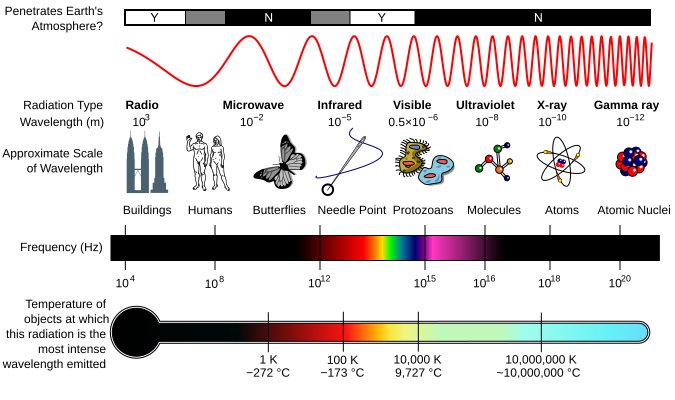
\includegraphics[width=\textwidth]{bilder/spektrum.png}
	\caption{The electromagnetic spectrum with typical applications. Source: Wikimedia Commons}
	\label{fig:em_spektrum}
\end{figure}

\subsubsection{Frequency, Wavelength, and Energy Ranges}

\begin{table}[H]
	\centering
	\scriptsize
	\resizebox{0.95\textwidth}{!}{
		\begin{tabular}{|l|c|c|c|}
			\hline
			\textbf{\raisebox{-0.2ex}{Region}} & \textbf{\raisebox{-0.2ex}{Frequency}} & \textbf{\raisebox{-0.2ex}{Wavelength}} & \textbf{\raisebox{-0.2ex}{Photon energy}} \\
			\hline
			Radio waves      & \SI{1e3}{}–\SI{1e8}{Hz} & km – m & \(\sim\)\SI{1e-9}{eV} \\
			Microwaves       & \SI{1e8}{}–\SI{1e11}{Hz} & m – mm & \(\sim\)\SI{1e-6}{eV} \\
			Infrared         & \SI{1e11}{}–\SI{4e14}{Hz} & mm – \SI{750}{nm} & \SI{1e-3}{eV} – \SI{1}{eV} \\
			Visible light    & \SI{4e14}{}–\SI{8e14}{Hz} & \SI{750}{nm} – \SI{380}{nm} & \SI{1.6}{eV} – \SI{3.3}{eV} \\
			Ultraviolet      & \SI{8e14}{}–\SI{3e16}{Hz} & \SI{380}{nm} – \SI{10}{nm} & up to \SI{100}{eV} \\
			X-rays           & \SI{3e16}{}–\SI{3e19}{Hz} & \SI{10}{nm} – \SI{0.01}{nm} & \SI{100}{eV} – \SI{100}{keV} \\
			Gamma rays       & >\SI{3e19}{Hz} & < \SI{0.01}{nm} & > \SI{100}{keV} \\
			\hline
		\end{tabular}
	}
	\caption{Typical regions of the electromagnetic spectrum with frequency, wavelength, and energy}
	\label{tab:spektrum}
\end{table}

\subsubsection{Applications Across the Spectrum}

Typical applications in different spectral regions:
\begin{itemize}
	\item \textbf{Radio waves:} broadcasting, radio communication, MRI
	\item \textbf{Microwaves:} mobile networks, WLAN, microwave oven
	\item \textbf{Infrared:} remote controls, thermography
	\item \textbf{Visible:} optics, photography, biological vision
	\item \textbf{UV:} sunburn, disinfection (UV-C)
	\item \textbf{X-ray:} medical imaging, materials testing
	\item \textbf{Gamma:} radiation therapy, astrophysics
\end{itemize}

\begin{tcolorbox}[hinweisbox,title=Takeaways on the Electromagnetic Spectrum]
	\label{box:Fazit zum elektro}
	\textbf{Physical takeaways:}
	\begin{itemize}
		\item The electromagnetic spectrum spans waves of all frequencies – from radio to gamma.
		\item Photon energy increases with increasing frequency (or decreasing wavelength) according to \(E = h \nu = \tfrac{hc}{\lambda}\).
		\item The transition to \textbf{ionizing radiation} typically begins in the UV, at photon energies around \SI{10}{\electronvolt}.
	\end{itemize}
	\vspace{0.5em}
	\textbf{Didactic takeaways:}
	\begin{itemize}
		\item Placing typical applications – e.g., mobile networks, microwaves, UV disinfection, X-ray diagnostics – in the spectrum clarifies their physical and biological effects.
		\item A visual link between frequency, wavelength, energy, and biological relevance is especially helpful.
		\item \textbf{Rule of thumb:} the shorter the wavelength, the higher the photon energy – and the greater the potential for biological damage.
	\end{itemize}
\end{tcolorbox}
\newpage
\noindent

\subsection{Masslessness and Propagation at the Speed of Light}\index{Masslessness}\index{Speed of light}

\subsubsection{No Rest Mass – Yet Energy and Momentum}

The photon has no rest mass, i.e., $m_0 = 0$. Nevertheless, it carries energy and momentum.\index{Energy} The photon energy (Planck–Einstein) is
$$
E = h \nu
$$
and the momentum follows as
$$
p = \frac{E}{c} = \frac{h\nu}{c} = \frac{h}{\lambda}
$$
Thus the photon does not contradict relativity – on the contrary: these relations are direct consequences of special relativity for massless particles.

\subsubsection{What If the Photon Had a Tiny Mass?}

\paragraph{Relativistic energy:} If the photon were not exactly massless, one would have to use the general relativistic energy formula
$$
E = \gamma m_0 c^2 = \frac{m_0 c^2}{\sqrt{1 - \frac{v^2}{c^2}}}
$$
and the momentum
$$
p = \gamma m_0 v
$$
Then the simple relation $E = pc$ would no longer be exact; instead
$$
E^2 = (pc)^2 + (m_0 c^2)^2
$$
(A detailed mathematical discussion for massless and hypothetically massive photons is given in Appendix~A, Sec.~\ref{anhangA:masse}.)
\newpage
\noindent
\subsubsection*{Physical Consequences:}
\phantomsection
\begin{itemize}
	\item The speed of light would no longer be the same for all photons.
	\item The speed would depend on energy (frequency) $\Rightarrow$ violation of Lorentz invariance.
	\item Long-wavelength light would travel more slowly than short-wavelength light.
	\item Coulomb's law would have to be modified $\Rightarrow$ the range of the electric force would be finite.
\end{itemize}

\paragraph{Experimental Bounds:}
Precise measurements show: if the photon has a mass, it must be extremely small:
$$
m_\gamma < 10^{-54}~\text{kg} \approx 10^{-18}~\text{eV}/c^2
$$
\index{Photon mass}
\textbf{This number} $10^{-54}~\text{kg}$ \textbf{is not a law of nature nor a theoretical prediction}, but an upper bound inferred from many experiments and observations – under the hypothesis that the photon might have a mass. No such tiny deviations have been observed.

\begin{figure}[H]
	\centering
	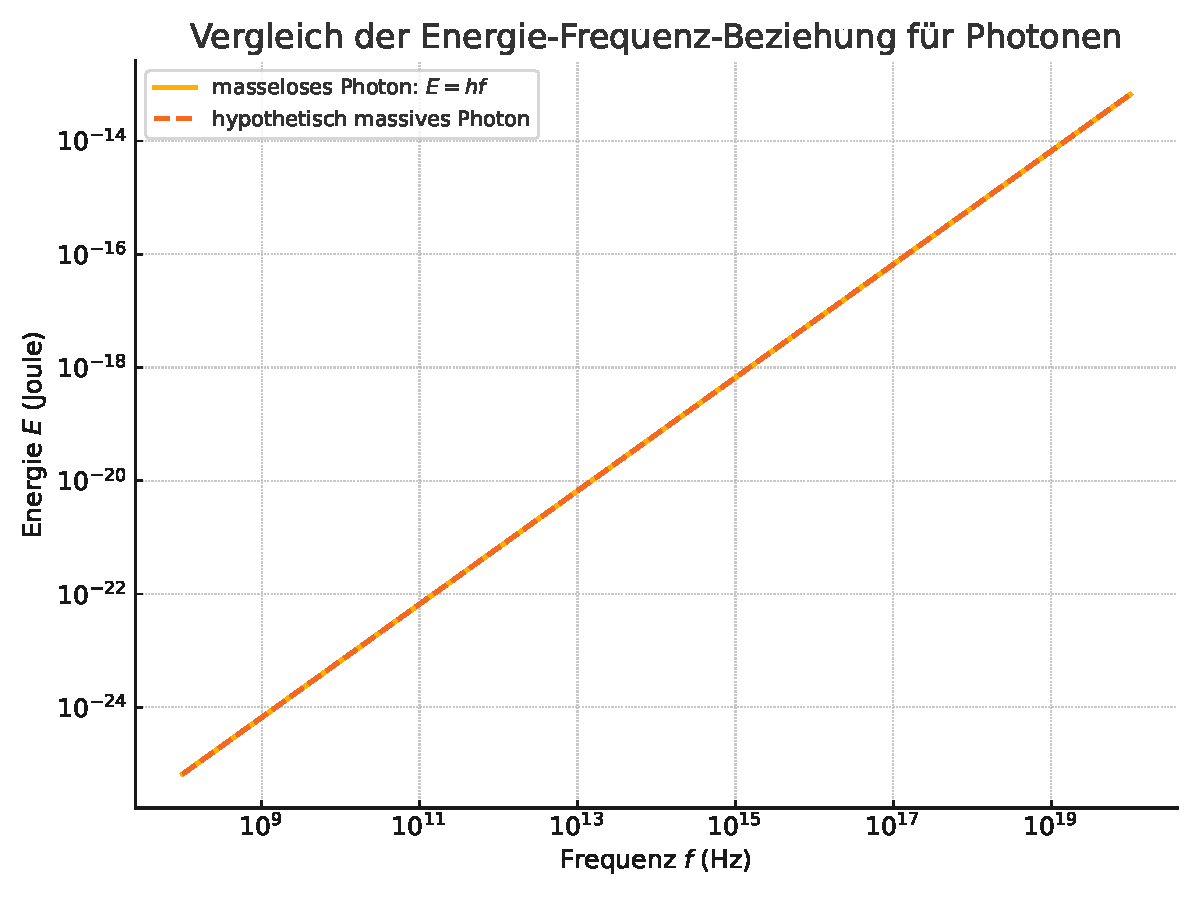
\includegraphics[width=0.85\textwidth]{bilder/photon_energie_vergleich_didaktisch.pdf}
	\caption{Didactic comparison of the energy–frequency relation \( E(f) \) for a massless photon (blue) and a hypothetical massive photon with exaggerated mass (red, dashed).}
	\label{fig:energie_f_masselos_massiv}
\end{figure}
\vspace{1em}
\begin{tcolorbox}[hinweisbox, title=Why No Difference Is Visible in the Plot]
	\label{box:Warum sieht man}
	The $E(f)$ relation is shown for massless and (exaggerated) massive photons. Because the experimental upper bound on the photon mass is so tiny ($m_\gamma < 10^{-54}$ kg), the two curves are practically indistinguishable even on log–log scales. \\[1ex]
	\textbf{This lack of deviation strongly supports the photon’s masslessness.}
\end{tcolorbox}
\vspace{1em}
\begin{tcolorbox}[hypobox, title={What if the Photon Had a Mass?}]
	\label{box:was wäre wenn}
	If the photon had even a tiny mass ($m_\gamma > 0$), then:
	\begin{itemize}
		\item It would travel more slowly than the speed of light ($v < c$),
		\item The energy–frequency relation would not be $E=hf$, but
		$$
		E = \sqrt{(hf)^2 + (m_\gamma c^2)^2}\,,
		$$
		\item The speed of light would not be universal – e.g., long-wavelength light would be slower than short-wavelength light,
		\item Coulomb’s law would be \emph{screened} – electric fields would have finite range.
	\end{itemize}
	Since none of this is observed, the photon is, with overwhelming evidence, truly massless.
\end{tcolorbox}
\vspace{1em}
\newpage
\noindent
\subsubsection{Why Would \( E = h f \) Fail for a Massive Photon?}

The formula $E = hf$ holds exactly only for massless particles. If the photon had mass, one would have
$$
E = \sqrt{(hf)^2 + (m_\gamma c^2)^2} \; > \; hf\,,
$$
so the energy would not depend on frequency alone – something that would be experimentally detectable.

\paragraph{Confirmed Experiments:}
\begin{itemize}
	\item Photoelectric effect
	\item Compton effect
	\item Spectral lines and laser spectroscopy
	\item Quantum optics and precision QED experiments
\end{itemize}
All confirm, to high precision, the relation $E = hf$. No systematic deviation has ever been found.
\vspace{1em}
\begin{tcolorbox}[physikbox, title=Conclusion: Why the Photon Is Massless]
	\label{box:Warum das Photon}
	\begin{itemize}
		\item The photon has no rest mass ($m_0 = 0$) but does have energy and momentum.
		\item It necessarily propagates at the speed of light: $v = c$.
		\item Only under this condition do $E = pc$ and $E = hf$ hold.
		\item If $m_\gamma > 0$, numerous observations and special relativity would be contradicted.
	\end{itemize}
\end{tcolorbox}
\vspace{1em}

\newpage
\noindent
\subsection{Spin and Polarization}\index{Spin}\index{Polarization}\index{Boson}\index{Helicity}

\subsubsection{Spin of the Photon}

In quantum mechanics, \textbf{spin} is a fundamental property of elementary particles – comparable to an intrinsic angular momentum. Unlike classical rotation, spin does not refer to literal spinning in space; it is a purely quantum property with discrete values.

\vspace{0.5em}
\textbf{Photons have spin 1} and thus belong to the class of \textit{bosons}. While half-integer spin particles (like electrons with spin $1/2$) are fermions and obey the Pauli principle, bosons can occupy the same quantum state – a principle with fundamental consequences for light, e.g., laser amplification.\index{Fermion}\index{Pauli principle}\index{Laser}
\vspace{1em}
\begin{tcolorbox}[physikbox, title=Properties of Photon Spin]
	\label{box:Eigenschaften des}
	\begin{itemize}
		\item Photons have \textbf{spin 1} but no rest mass.
		\item Only two measurable spin states exist: \textbf{helicity $+1$ and $-1$}.
		\item The \textbf{spin direction} is always along the photon’s direction of motion.
	\end{itemize}
\end{tcolorbox}
\vspace{1em}
The restriction to only two spin states is a direct consequence of the photon’s \textbf{masslessness}. In contrast to massive spin‑1 particles (e.g., the Z boson), there is no rest frame for the photon; thus the longitudinal ($0$) spin state is absent. Only the two transverse helicity modes $\pm 1$ remain.\index{Z boson}

(A formal derivation of the allowed photon helicities is given in Appendix~A, Sec.~\ref{anhangA:helizitaet}.)

\newpage
\noindent
\textbf{Helicity} is the projection of spin onto the direction of motion:
\begin{itemize}
	\item \textbf{Helicity $+1$:} right‑circularly polarized light.
	\item \textbf{Helicity $-1$:} left‑circularly polarized light.
\end{itemize}

\begin{figure}[H]
	\centering
	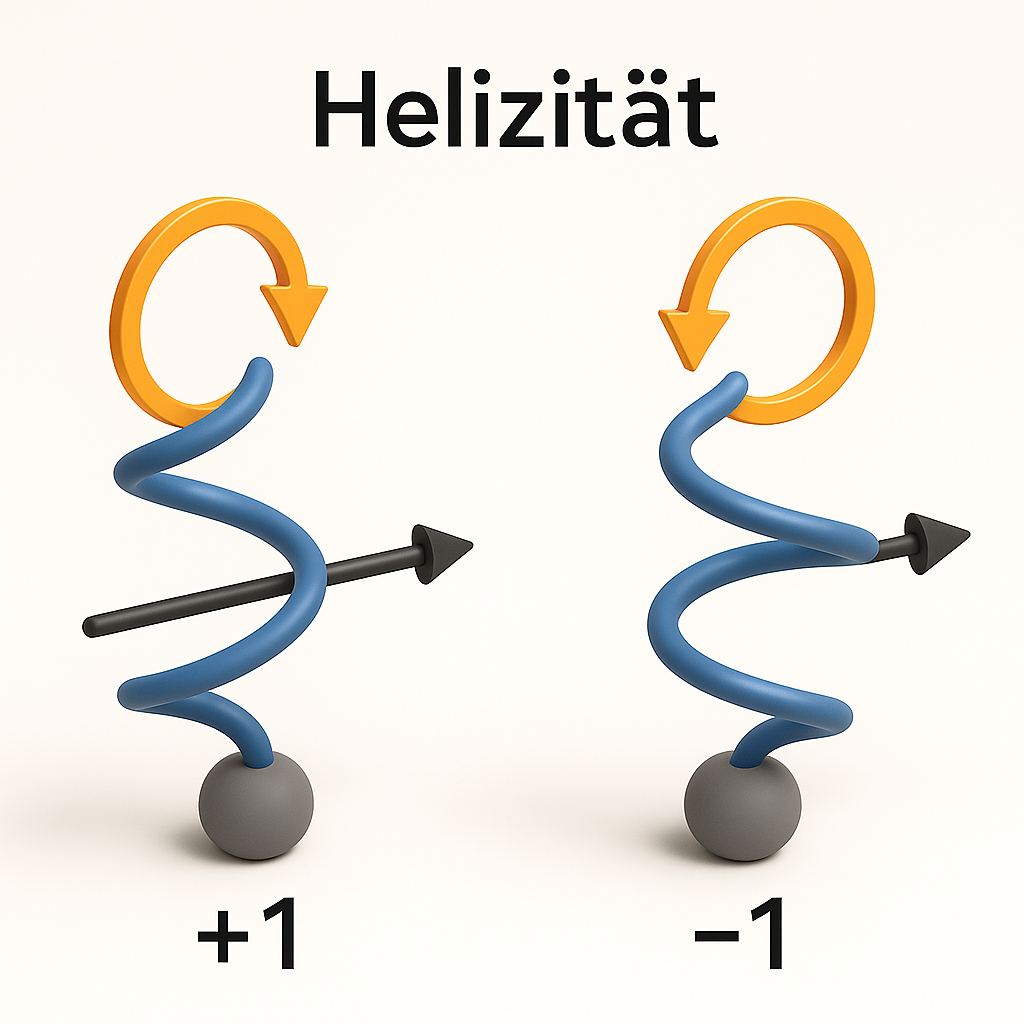
\includegraphics[width=0.65\textwidth]{bilder/Helizitaet.png}
	\caption{Visualization of photon helicity. Left: helicity $+1$ (right‑circular), right: helicity $-1$ (left‑circular). Orange arrows indicate spin (field rotation), black arrows indicate propagation direction.}
	\label{fig:helizitaet}
\end{figure}

\begin{tcolorbox}[physikbox, title=Comment on the Illustration]
	\label{box:Kommentar zur Darstellung}
	The spiral depicts how the electric field vector rotates for circular polarization. The photon travels straight along the propagation direction (momentum arrow). The spiral shows rotation of the field – not the photon’s path. This distinction is crucial for understanding helicity.
\end{tcolorbox}
\vspace{1em}
These two states underpin \textit{circular polarization}, discussed next.

\newpage
\noindent
For comparison:
\begin{itemize}
	\item An \textbf{electron} has spin $1/2$ with two states (up/down).
	\item A \textbf{Z boson} (massive, spin 1) exhibits three states: $-1$, $0$, $+1$.
	\item The \textbf{photon} (massless, spin 1) exhibits only $-1$ and $+1$ – the $0$ state is absent.
\end{itemize}
\vspace{1em}
\begin{tcolorbox}[physikbox, title=Didactic Rule of Thumb]
	\label{box:didaktischerMerksatz}
	Massless spin‑1 particles such as photons possess only two helicity states: \textbf{$\pm1$}. A longitudinal ($0$) state does not exist because no rest frame can be defined.
\end{tcolorbox}
\vspace{1em}

\subsubsection*{Conclusion}
\phantomsection
The photon’s spin fundamentally differs from that of massive particles. As a massless spin‑1 particle, the photon has only two helicity states: $+1$ and $-1$. A longitudinal helicity‑0 state is excluded because no rest frame exists.

\vspace{0.5em}
Spin can thus only be considered along the direction of motion – it manifests as helicity:
\begin{itemize}
	\item Helicity $+1$: spin aligned with motion (right‑circular)
	\item Helicity $-1$: spin opposite to motion (left‑circular)
\end{itemize}
A classical picture of literal rotation is inapplicable. Spin is an intrinsic quantum property that appears, for photons, as circular polarization.

\subsubsection{Polarization as a Macroscopic Manifestation of Spin}

Polarization is an observable phenomenon directly linked to the quantum spin of photons. While spin is an intrinsic property of each photon, polarization describes the collective state of a light field – i.e., many photons together.

\vspace{0.5em}
Classically, polarization is the orientation of the electric field vector of an electromagnetic wave. This vector oscillates transverse to the direction of propagation and can take different orientations and rotations:
\begin{itemize}
	\item \textbf{Linearly polarized light:} the electric field oscillates in a fixed direction (e.g., vertical or horizontal).
	\item \textbf{Circularly polarized light:} the field vector rotates at constant amplitude – clockwise (right‑circular) or counterclockwise (left‑circular).
	\item \textbf{Elliptically polarized light:} the most general case – the field vector traces an ellipse.
\end{itemize}
\index{Linearly polarized light}\index{Circularly polarized light}\index{Elliptically polarized light}

\vspace{0.5em}
In quantum optics, polarization corresponds to the collective helicity content of many photons.\index{Quantum optics} A fully right‑circularly polarized field consists of photons with helicity $+1$, a left‑circular field of photons with $-1$. Linear polarization arises from a quantum superposition of both helicity states:
$$
|\text{linear}\rangle = \frac{1}{\sqrt{2}} \bigl( |+1\rangle + |-1\rangle \bigr)
$$
(A more detailed treatment using Dirac notation and Jones vectors is given in Appendix~A, Sec.~\ref{anhangA:polarisation}.)
\vspace{1em}
\begin{tcolorbox}[physikbox, title=Superposition and Polarization]
	\label{box:Superposition}
	A linearly polarized photon is a quantum superposition of the two helicity states $|+1\rangle$ and $|-1\rangle$. This superposition leads to the fixed oscillation direction of the electric field.
\end{tcolorbox}

\vspace{0.5em}
Thus polarization is a directly observable consequence of photon spin. In many experiments – e.g., with polarizers, polarization cameras, or double-slit setups using polarized light – polarization appears as a macroscopic manifestation of quantum states.\index{Polarizer}
\vspace{1em}
\begin{tcolorbox}[physikbox, title=Superposition and Polarization]
	\label{box:Superposition und Polarisation}
	A linearly polarized photon is in a quantum superposition of the two helicity states $|+1\rangle$ (right‑circular) and $|-1\rangle$ (left‑circular):
	$$
	|\text{linear}\rangle = \frac{1}{\sqrt{2}} \left( |+1\rangle + |-1\rangle \right).
	$$
	This implies:
	\begin{itemize}
		\item The photon has no definite helicity.
		\item It is simultaneously in $|+1\rangle$ and $|-1\rangle$ with equal amplitude and fixed phase.
		\item The fixed oscillation direction (linear polarization) arises from this coherent superposition.
		\item Measuring helicity destroys the superposition: the photon is found with helicity $+1$ or $-1$ – never both at once.
	\end{itemize}
	Polarization is therefore more than a field direction – it is the expression of a quantum state that is fully captured only via superposition.
\end{tcolorbox}

\subsubsection{Measuring and Detecting Polarization}

Polarization is a macroscopic observable consequence of the photon’s quantum spin structure. Various optical methods are available – from simple polarizers to precise single‑photon detectors in quantum optics.

\vspace{0.5em}
\textbf{Linear polarization} can be tested classically with two polarizers: a linearly polarized beam passes a second polarizer (the “analyzer”). The transmitted intensity varies with the relative angle according to \textbf{Malus’s law}:\index{Malus’s law}
$$
I = I_0 \cos^2\theta
$$
where \( \theta \) is the angle between the incident polarization and the analyzer axis.

\vspace{0.5em}
\textbf{Circular polarization} is revealed by combining a linear polarizer with a quarter‑wave plate,\index{Quarter-wave plate} which converts circular to linear polarization for analysis.

\vspace{0.5em}
\textbf{Single‑photon experiments} in quantum optics directly probe quantized polarization:
\begin{itemize}
	\item A photon impinges on a polarizer and is either transmitted or absorbed.
	\item Repeated measurements on identically prepared photons yield polarization statistics.
	\item These experiments show: polarization is a single‑photon phenomenon, not merely a classical wave effect.
\end{itemize}

\vspace{0.5em}
\textbf{Technical applications} abound:
\begin{itemize}
	\item LCD displays, polarized sunglasses, remote sensing
	\item Communications using polarization multiplexing (e.g., in fiber optics)
	\item Quantum communication with polarized single photons (QKD)
\end{itemize}
\index{QKD (quantum key distribution)}\index{Polarization multiplexing}

\begin{tcolorbox}[physikbox, title=What Polarization Reveals About Photons]
	\label{box:Was uns die}
	Polarization is not only a property of electromagnetic waves but a directly measurable result of photon spin. Polarization measurements allow fundamental statements about the states of single light quanta – up to and including entanglement in quantum physics.
\end{tcolorbox}
\index{Entanglement}

\subsection{Conclusion }\index{Conclusion}

Chapter~III has shown how light can be understood, from the quantum‑mechanical viewpoint, not only as an electromagnetic wave but also as a particle – the photon. This understanding unites classical concepts such as frequency and polarization with quantized properties such as energy, momentum, and spin.

\vspace{0.5em}
Key insights:
\begin{itemize}
	\item A photon’s energy is directly proportional to its frequency: \( E = h\nu \).
	\item A photon’s momentum is determined by its wavelength: \( p = \tfrac{h}{\lambda} \).
	\item Photons have spin~1 but, due to masslessness, only the helicity states $+1$ and $-1$ occur.
	\item The polarization of macroscopic light fields is a collective phenomenon rooted in the quantum states of many photons.
\end{itemize}

\vspace{0.5em}
These quantized properties of the photon will play a central role in Chapter~IV, where we explore the wave nature of particles and the particle nature of waves in the form of wave–particle duality.
